\section{WORLD MODELS} \label{approach}

In this paper, we aim to reproduce the world model developed by Ha and Schmidhuber \cite{1.0.0} for the \texttt{CarRacing-v0} environment and adapt the trained VAE and MDRNN to simplify the input state an Actor-Critic agent receives when trained online in the environment. Then, we will evaluate the performance of the Actor-Critic agent when trained with state simplification. This will be compared to the baseline for Actor-Critic agents trained from raw image states as well as a controller trained via CMA-ES from the original paper. We will also investigate the resulting improvement from a second iteration of training the VAE and MDRNN on additional policy sampled rollouts and then using this World Model to train Actor-Critic algorithms and the controller from before.

\subsection{VAE Model}

As the states sampled from the \texttt{CarRacing-v0} environment are high dimensional images, a VAE is used to compress an input state image $s_t$ into a latent feature vector $z_t$ with an encoder component which can also be reconstructed with a decoder component to observe the preserved features \cite{1.0.1} as shown in Figure \ref{fig:vae}. A VAE is ideal for this task as it learns to encode the most important sources of variation from the set of images trained on into a limited size representation of 32 units. We will use the same network architecture defined in the original paper \cite{1.0.0} for both iterations of training from random and policy sampled rollouts.

\begin{figure}[h]
	\centering
	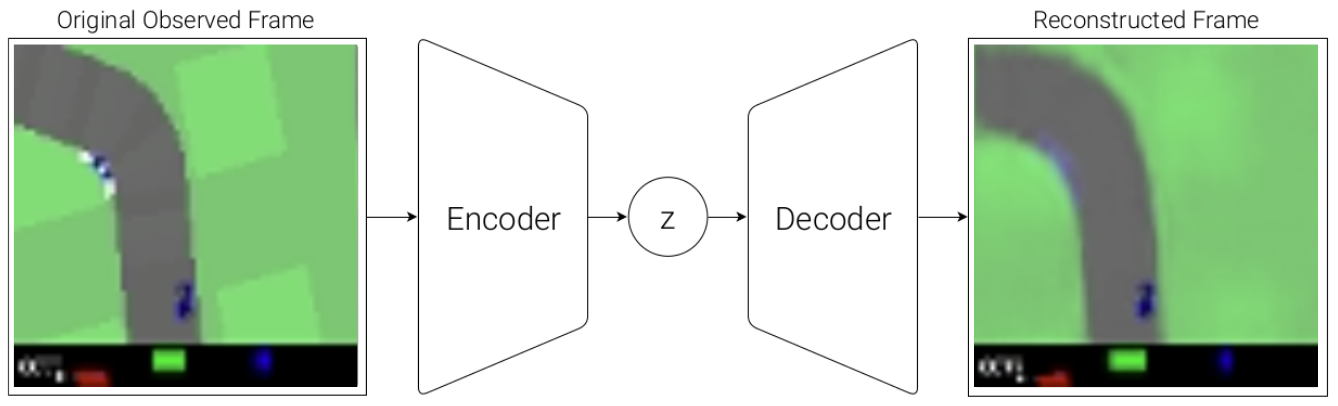
\includegraphics[width=0.49\textwidth]{images/vaes.png}
	\caption{Flow diagram of a VAE}\label{fig:vae}
\end{figure}

\subsection{MDRNN Model}

While the agent can access more important feature information about a state $s_t$ from a compressed latent vector $z_t$, it is only a static representation at a single point in time and doesn't contain temporal information such as the velocity of the car. Therefore, a Recurrent Neural Network (RNN) is used to encode dynamic information over a sequence of latent vectors. In \cite{1.0.0}, the RNN was used to predict the next state's latent representation $z_{t+1}$ from the current latent vector $z_t$, chosen action $a_t$ and its own internal hidden state $h_t$. As the distribution of the possible next states is often stochastic, the output of the RNN is passed to a Mixture-Density Network (MDN) \cite{1.2.1}, forming a Mixture-Density RNN (MDRNN) as shown in Figure \ref{fig:mdrnn}. 

\begin{figure}[h]
	\centering
	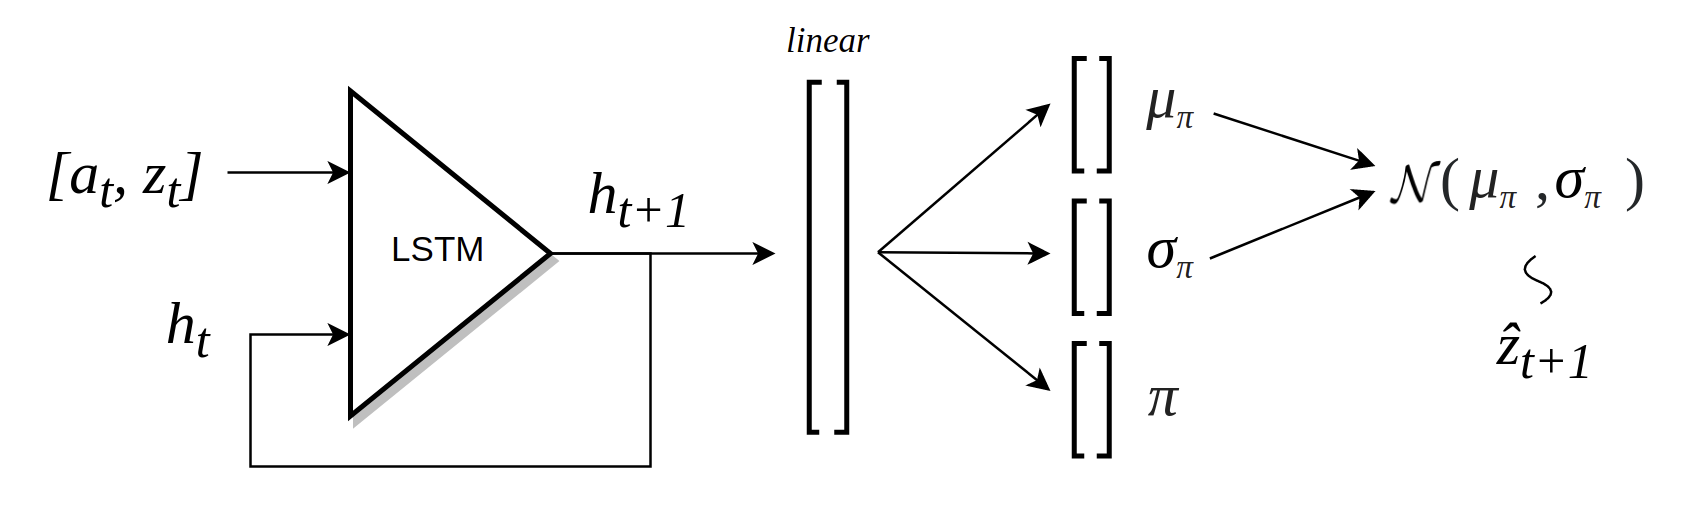
\includegraphics[width=0.5\textwidth]{images/mdrnn.png}
	\caption{Flow diagram of a MDRNN}\label{fig:mdrnn}
\end{figure}

Here, a Long-Short-Term-Memory (LSTM) network with a hidden size of 256 will be used as the RNN where the output hidden vector $h_{t+1}$ is passed through a fully connected linear layer and then split into three 5-length vectors representing the mean $(\mu)$, standard deviation $(\sigma)$, and mixing weights $(\pi)$, for each of 5 Gaussian distributions forming a mixture of Gaussians according to the mixing weights. Therefore, the MDRNN can be thought of as a function $M(a_t,z_t;h_t;\beta) \rightarrow h_{t+1},$ \textbf{$\mu$}, \textbf{$\sigma$}, \textbf{$\pi$} parameterized by $\beta$ \cite{1.2.0}. Given an experience tuple $(s_t, a_t, s_{t+1}, r_t, d_t)$, the latent states $z_t$ and $z_{t+1}$ can be obtained from a trained VAE's output from $s_t$ and $s_{t+1}$. Then with the probability $p(z_{t+1}|\mu,\sigma;\beta)$ of sampling $z_{t+1}$ from $\mu$ and $\sigma$, the loss function for training the MDRNN is:

\begin{dmath}
	L_M(\beta) = -\mathbb{E}_{(z,z') \sim VAE(\mathcal{E}),\ a \sim \mathcal{A},\ (\mu,\sigma,\pi) \sim M(a,z)} \\ \left[ \log \left( \sum^n_i \pi_i \ p(z'|\mu_i,\sigma_i;\beta) \right) \right] 
\end{dmath} 

The MDRNN is trained at each gradient step with a batch of 16 sequences of experience tuples having a sequence length of 32. Then, for predicting the hidden state from a single experience tuple, an LSTM cell is loaded with the trained weights and used within the MDRNN cell. The trained MDRNN along with the trained VAE make up the World Model network.

\subsection{Agent Model}

The role of the agent is to map input states to actions to select in a given input state. The original state $s_t$ produced from the environment is a 96x96x3 dimensional image which will be resized to 64x64x3, having a total of 12288 inputs. With the World Model consisting of the VAE and MDRNN, the compressed state vector $x_t = [z_t, h_t]$ is the concatenation of the latent vector $z_t$ of size 32 from the VAE and the hidden state $h_t$ of size 256 from the MDRNN, totaling 288 inputs. We will model three different approaches of training an agent to select actions optimally. The first will be a simplified implementation of the controller network in the original World Models paper \cite{1.0.0} using the compressed state vector $x_t$. Then, DDPG and PPO agents with similar network architectures will be trained first from raw image inputs $s_t$ as a baseline, and then using the compressed state vector $x_t$.

\subsubsection{CMA-ES Agent}

The original paper used a simple feed-forward network with a single layer mapping the compressed state input $x_t$ directly to the action vector $a_t$ of 3 continuous values for steering, acceleration, and braking. This can be represented as $a_t = W_c \cdot x_t + b_c$ where $W_c$ is the weight and $b_c$ is the bias for the single-layer network. The controller will be trained with the CMA Evolutionary Strategy with a smaller population size of 16 instead of 64 used previously in order to match the number of parallel agents per rollout across all agent models.

\subsubsection{DDPG and PPO Agent}

These agents will be tested first with raw 64x64x3 images $s_t$ as inputs to evaluate the baseline performance without a World Model providing a simplified state representation. Similar to the approach for learning Atari games from image inputs \cite{2.1.1}, each individual image will be converted to a single channel 64x64 grayscale frame which is then stacked on top of the previous frame to form an input size of 64x64x2, allowing for temporal information to be included in the difference between the two frames in sequence. Then, the architecture of the baseline actor and critic will consist of a convolutional component to reduce the 2D input to a vector which is then passed to a feed-forward component representing the respective objective output function. The convolutional component will have four convolutional layers with the same architecture as the encoder network in the VAE with the final output having a size of 512 representing the compressed state, denoted as $\hat{x}_t$, of the convolutional component. This is to mimic the encoder of the VAE in the World Model which can be thought of as being trained with the rest of the network. When trained with the World Model, the convolutional component will be replaced with a single fully connected layer transforming the input $x_t$ with 288 units to a size of 512 to have the same output size of the convolutional component.

The feed-forward component of the actor and the critic will take the rectified (ReLU) output of the convolutional or single layer of size 512 as input. For PPO, the critic representing the state value $V(s_t)$ will pass the input to a hidden layer of size 1024 with ReLU activation followed by a second hidden layer of size 1024 with ReLU activation, then finally to an output layer of size 1, being the scalar value $v_t$. For DDPG, the critic representing the state-action value function $Q(s_t,a_t)$ will also take an input action $a_t$ and pass it to a layer of size 512 before concatenating it with the state input which is then passed to the remaining layers as defined for PPO to obtain $q_t$. For the actor, the state input is passed through a hidden layer of size 256 with ReLU activation followed by a second hidden layer of size 256 with ReLU activation. The output to this layer will then be passed to two layers of size 3, representing the mean $(\mu_a)$ and standard deviation $(\sigma_a)$ for the Gaussian parameters of the next action to take. For DDPG, the resulting action will be calculated as $a_t = \mu_a + \epsilon \sigma_a$ where $\epsilon \sim \mathcal{N}(0,I)$. For PPO, the action is sampled from the Gaussian as $a_t \sim \mathcal{N}(\mu_a,\sigma_a^2)$.

Both the DDPG and PPO agents will be trained asynchronously with 16 agents acting in 16 different environments with parallel gradient updates using a learning rate of 0.0001 as this is known to speed up training efficiency \cite{2.2.1}. For DDPG, an experience replay buffer of max length 100000 will be used to store experience tuples which are sampled in batches of 32 for each gradient step. A Brownian noise process is used to ensure exploration where the scale of noise is reduced from 1.0 to a minimum of 0.1 at a decay rate of 0.99 after each episode. For PPO, the clip ratio $\epsilon$ is decayed from 0.1 to a minimum of 0.01 at a decay rate of 0.995 after each batch update. Gradient updates are taken every 20 time-steps with a batch size of 5 over 4 epochs. An entropy prioritization weight of 0.005 is used for exploration. The complete implementation of the networks is available on Github at \cite{Git}.